\scanpage{220}
% archive sheet number: 219

\mspage{- 12 -} \hfill n\textsuperscript{o}370

4) Supposons $G$ unimodulaire. Soit $\mu$ une mesure de Haar sur $G$. On a

\[
\gamma(s)\mu=\delta(s)\mu=\check{\mu}=\mu. \tag*{(26)}
\]

Si $f$ est $\mu$-intégrable sur $G$, les translatées à gauche et à droite de $f$ sont $\mu$-intégrables ainsi que $\check f$, et on a

\[
\int f(sx)\,\mathrm{d}\mu(x)=\int f(xs)\,\mathrm{d}\mu(x)=\int f(x^{-1})\,\mathrm{d}\mu(x)=\int f(x)\,\mathrm{d}\mu(x). \tag*{(27)}
\]

Si $A$ est une partie $\mu$-intégrable de $G$, $sA$, $As$ et $A^{-1}$ sont $\mu$-intégrables, et

\[
\mu(sA)=\mu(As)=\mu(A^{-1})=\mu(A). \tag*{(28)}
\]

% Pale pencil traces to the left of (28).
\figure{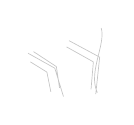
\begin{tikzpicture}[x=1cm,y=1cm,gray!45,line width=.25pt]
\draw (0,.58) -- (.34,.39) -- (.45,.03) (.07,.60) -- (.36,.41) -- (.40,.14) (.03,.47) -- (.24,.34) -- (.29,.09);
\draw (.52,.74) -- (.91,.53) -- (.86,.06) (.49,.66) -- (.83,.47) -- (.80,.12) (.88,.08) .. controls (.76,.34) and (.99,.69) .. (.93,.90);
\end{tikzpicture}}

On a des propriétés analogues pour l'intégrale essentielle.

PROPOSITION 2.- \uline{S'il existe dans} $G$ \uline{un voisinage compact} $V$ \uline{de} $e$ \uline{invariant par automorphismes intérieurs}, \uline{alors} $G$ \uline{est unimodulaire}.

En effet, soit $\mu$ une mesure de Haar à gauche sur $G$. On a, pour tout $s\in G$, $\mu(V)=\mu(s^{-1}Vs)=\Delta_G(s)\mu(V)$, d'où $\Delta_G(s)=1$ puisque $0<\mu(V)<+\infty$.

On en déduit aussitôt :

COROLLAIRE.- \uline{Si} $G$ \uline{est discret}, \uline{ou compact}, \uline{ou commutatif}, $G$ \uline{est unimodulaire}.

Ceci est d'ailleurs trivial lorsque $G$ est \uline{commutatif}. Notons aussi que, si $G$ est \uline{discret}, la mesure sur $G$ pour laquelle chaque point est de masse $1$ est évidemment une mesure de Haar à gauche et à droite sur $G$, qu'on appelle mesure de Haar \uline{normalisée} sur $G$. Si $G$ est \uline{compact}, il existe une mesure de Haar $\mu$ et une seule sur $G$ telle que $\mu(G)=1$ ; on l'appelle la mesure de Haar \uline{normalisée} de $G$. Les deux conventions précédentes ne concordent pas lorsque $G$ est à la fois discret et compact, c'est-à-dire fini ; quand on sera dans ce cas, on précisera toujours explicitement ce qu'on entend par mesure de Haar normalisée.

Un sous-groupe, un groupe quotient d'un groupe unimodulaire ne sont pas toujours unimodulaires (\S\ 2, exerc. 5). Cf., toutefois, le \S\ 2, prop. 10.

\textsuperscript{$\ast$}Nous verrons plus tard que les groupes de Lie connexes semi-simples ou nilpotents sont unimodulaires.\textsubscript{$\ast$}
